% !TeX program = lualatex
\documentclass[10pt,aspectratio=169]{beamer}
\usepackage[haranoaji,deluxe]{luatexja-preset}
\usepackage{graphicx}
\usepackage{tikz}
\renewcommand{\kanjifamilydefault}{\gtdefault}
\renewcommand{\familydefault}{\sfdefault}

\definecolor{Ink}{HTML}{142C43}
\definecolor{Muted}{HTML}{647382}
\definecolor{Past}{HTML}{A5673F}
\definecolor{Now}{HTML}{087F83}
\definecolor{Pale}{HTML}{F0F4F6}
\definecolor{Gold}{HTML}{D69A22}

\setbeamercolor{normal text}{fg=Ink,bg=white}
\setbeamercolor{structure}{fg=Now}
\setbeamertemplate{navigation symbols}{}
\setbeamersize{text margin left=9mm,text margin right=9mm}
\setbeamertemplate{footline}{\hspace{9mm}\makebox[142mm]{\tiny\color{Muted}大分大学での近況報告\hfill マルチメディア研究会2026夏\hspace{5mm}\insertframenumber/\inserttotalframenumber}\vspace{2mm}}
\setlength{\parindent}{0pt}

\newcommand{\head}[3]{%
 {\color{Now}\fontsize{13}{16}\selectfont\bfseries #1\par}
 \vspace{1.2mm}
 {\color{Muted}\fontsize{8.5}{11}\selectfont\bfseries SECTION #2\quad/\quad #3\par}
 \vspace{1.7mm}{\color{Ink}\hrule height .4pt}\vspace{2.4mm}}
\newcommand{\pair}[4]{%
 \begin{columns}[T,onlytextwidth]
 \begin{column}{.475\textwidth}
 {\color{Past}\fontsize{10}{12}\selectfont\bfseries #1\par}\vspace{1.2mm}#2
 \end{column}
 \begin{column}{.475\textwidth}
 {\color{Now}\fontsize{10}{12}\selectfont\bfseries #3\par}\vspace{1.2mm}#4
 \end{column}
 \end{columns}}
\newcommand{\bigtext}[1]{{\fontsize{14}{17}\selectfont\bfseries #1\par}\vspace{1.2mm}}
\newcommand{\body}[1]{{\fontsize{9.3}{13}\selectfont #1\par}}
\newcommand{\smalltext}[1]{{\fontsize{7.4}{10}\selectfont\color{Muted}#1\par}}
\newcommand{\bullets}[1]{{\fontsize{8.8}{12}\selectfont #1\par}}
\newcommand{\lineitem}[1]{\textbullet\ #1\par\vspace{.45mm}}
\newcommand{\visual}[3]{%
 \vspace{1.5mm}\IfFileExists{assets/#1}{%
 \begin{minipage}[c][#2][c]{\linewidth}\centering
 \includegraphics[width=\linewidth,height=#2,keepaspectratio]{assets/#1}
 \end{minipage}}{%
 \begingroup\setlength{\fboxsep}{2mm}\colorbox{Pale}{%
 \begin{minipage}[c][\dimexpr#2-4mm\relax][c]{\dimexpr\linewidth-4mm\relax}
 \centering\color{Muted}\fontsize{8}{11}\selectfont #3
 \end{minipage}}\endgroup}\par}
\newcommand{\pending}[1]{\vspace{1.2mm}\smalltext{［要追記］#1}}
\newcommand{\bridge}[1]{\vfill{\color{Muted}\fontsize{7.5}{10}\selectfont #1\par}}
\newcommand{\sessionpaper}[3]{%
 {\fontsize{6.4}{7.5}\selectfont\color{Now}\bfseries 10-2P-#1\hfill
  \color{Past}第一著者：#2\par}%
 \vspace{.25mm}
 {\fontsize{5.7}{6.9}\selectfont\color{Ink}#3\par}%
 \vspace{.65mm}{\color{Ink!16}\hrule height .35pt}\vspace{.7mm}}

\begin{document}

\begin{frame}[plain]
\begin{columns}[c,onlytextwidth]
\begin{column}{.53\textwidth}
 {\color{Now}\fontsize{9}{12}\selectfont\bfseries マルチメディア研究会2026夏\par}
 \vspace{5mm}
 {\fontsize{25}{31}\selectfont\bfseries AIで研究は速くなった。\\でもGPUは1枚200万円超。\par}
 \vspace{5mm}
 {\color{Past}\fontsize{12}{16}\selectfont\bfseries 大分大学で研究室を始めて2年半\par}
 \vspace{7mm}
 {\fontsize{11}{15}\selectfont\bfseries 大知 正直\par}
 \vspace{1mm}
 {\fontsize{8.5}{12}\selectfont 大分大学理工学部DX人材育成プログラム\par}
 \vspace{5mm}
 \smalltext{2026年9月20日\quad 電気通信大学}
\end{column}
\begin{column}{.41\textwidth}
 \visual{poster-lab-gathering.png}{62mm}{写真：現在の研究室}
\end{column}
\end{columns}
\end{frame}

\begin{frame}[t]
\head{大分に来て2年半、制度も研究室も大学院も同時に始まりました}{01}{近況と沿革}
\pair{2024年}{
 \bigtext{制度と研究室がスタート}
 \bullets{
  \lineitem{4月：DX人材育成プログラム新設、学部定員40名}
  \lineitem{5月：大知が着任}
  \lineitem{10月：3年生4名が研究室へ配属}}
 \visual{02-bcore-opening.png}{24mm}{写真：B-Core開所式}
}{2025--2026年}{
 \bigtext{大学院と企業へ広がる}
 \bullets{
  \lineitem{2025年4月：大学院とB-Coreが始動。初年度9名、社会人2名}
  \lineitem{7月：企業交流イベント／9月：研究室合宿}
  \lineitem{10月：3年生3名が配属}
  \lineitem{2026年3月：今泉先生が異動（岩上さんの大学の教授）}}
 \visual{03-first-cohort.png}{19mm}{写真：大学院1期生}
}
\end{frame}

\begin{frame}[t]
\head{授業と企業調整を、研究として着地するまで担当しています}{01}{大学院教育}
\pair{データサイエンス特論1（M1）}{
 \bigtext{分析して、説明する}
 \bullets{
  \lineitem{データの収集、分析、可視化}
  \lineitem{学生自身がテーマを設定}
  \lineitem{分析結果をポスターへまとめる}
  \lineitem{最終ポスター発表会で説明する}}
 \visual{04-practice-poster.png}{23mm}{写真：最終ポスター発表会}
}{データサイエンス実践演習}{
 \bigtext{企業課題を研究へ変える}
 \bullets{
  \lineitem{M1後半からM2前半まで約1年}
  \lineitem{企業の実データと実課題}
  \lineitem{企業と学生のマッチング}
  \lineitem{データ条件、定例会、進捗、期待値を調整}
  \lineitem{特定課題研究として完成させる}}
 \smalltext{産学融合は、企業と学生を会わせれば始まるわけではない。}
}
\end{frame}

\begin{frame}[t]
\head{県立高校出身の理事から宿題が降り、小学生にはカードを配ります}{02}{地域貢献}
\pair{高校ではなく大学理事から}{
 \bigtext{地域貢献の「指令」}
 \bullets{
  \lineitem{県立高校出身の大学理事から現場へ降りてくる}
  \lineitem{国立大なのに、オープンキャンパスは年7回}
  \lineitem{「探究の授業をお願いします」}
  \lineitem{「研究室体験をお願いします」}
  \lineitem{問い、収集、分析、表現まで支援する}}
 \visual{poster-highschool-class.png}{23mm}{写真：高校での授業}
 \smalltext{なぜ理事から研究室へ指令が来るのかは、今も謎。}
 \smalltext{出典：文部科学省「総合的な学習（探究）の時間」}
}{こちらから仕掛ける活動}{
 \bigtext{小学生へカードを配る}
 \bullets{
  \lineitem{AI手法、データ、GPUをカード化}
  \lineitem{難しい用語へ、遊びから入ってもらう}
  \lineitem{学祭で小学生へ配布する計画}
  \lineitem{将来の志願者になる前から人気を取る}}
 \visual{poster-card-game.png}{28mm}{画面：データサイエンスカードゲーム}
}
\end{frame}

\begin{frame}[t]
\head{高校生向けPRより、大分にいる社会人を大学院へ呼びたい}{02}{社会人の受け入れ}
\pair{高校生は地元へ戻るという見立て}{
 \bigtext{地元回帰は強まるという見立て}
 \bullets{
  \lineitem{少子化でも、地方世帯の所得は増えていない}
  \lineitem{県外進学の学費・家賃・移動負担は重くなる}
  \lineitem{進学先はむしろ地元へ戻ると考えている}
  \lineitem{オープンキャンパス年7回の限界効用は低い}
  \lineitem{高校生PRは義務としてやるが、成長戦略にはしない}}
}{会社所属のまま2名が入学}{
 \bigtext{大分大は「大分の東大」}
 \bullets{
  \lineitem{大分で高度な理系を学び直す場所は少ない}
  \lineitem{学部卒で就職し、学ぶ機会を失った社会人がいる}
  \lineitem{大分ガスとクラウン建築設計事務所から各1名}
  \lineitem{会社に所属したまま大学院へ入学}
  \lineitem{配管故障の推定／建物の耐震補強を研究題材に}
  \lineitem{会社の課題を研究へ変え、知見を会社へ戻す}}
 \visual{poster-oita-hub.png}{23mm}{図：大分大学を中心にした地域の知的循環}
}
\bridge{社会人受け入れ ＝ 学生確保 ＋ 産学融合 ＋ 地域企業への知見還元}
\end{frame}

\begin{frame}[t]
\head{DAIBフェローになり、「AIの人」として地域へ名刺を配っています}{03}{地域でのAIキャラ}
\pair{県庁のAI連携団体}{
 \bigtext{DAIBのフェローをしています}
 \bullets{
  \lineitem{大分県のDigital \& AI Innovation Bridge}
  \lineitem{県内事業者とAI・ロボティクスの専門家をつなぐ}
  \lineitem{大学でも「AIの人」として通るようになってきた}
  \lineitem{技術相談や企業課題が集まる立場を作る}}
 \visual{poster-daib.png}{17mm}{DAIBロゴ}
}{名刺配りから研究へ}{
 \bigtext{とにかく接点を増やす}
 \bullets{
  \lineitem{地域企業へ名刺を配る}
  \lineitem{県庁職員へ名刺を配る}
  \lineitem{教育委員会へも名刺を配る}
  \lineitem{高校の探究、実践演習、技術相談へつなぐ}
  \lineitem{長期テーマは社会人学生・共同研究へ育てる}}
 \visual{poster-data-ai-social.png}{27mm}{図：データ収集からAI、社会実装まで}
}
\bridge{名刺 → 相談 → 授業・実践演習 → 社会人学生・共同研究}
\end{frame}

\begin{frame}[t]
\head{AIは速い。GPUは200万円超、10万円から大学資産です}{03}{計算資源と資産管理}
\pair{AIで短縮できた作業}{
 \bigtext{調査・実装・実験・執筆}
 \bullets{
  \lineitem{文献と背景の調査}
  \lineitem{コード作成とエラー対応}
  \lineitem{実験の自動化と結果整理}
  \lineitem{論文の下書きと修正}}
}{値段と管理は重くなる}{
 {\color{Gold}\fontsize{24}{28}\selectfont\bfseries RTX PRO 6000\\200万円超\par}\vspace{2mm}
 \bullets{
  \lineitem{円安がGPU価格を直撃}
  \lineitem{大学は10万円以上を資産登録}
  \lineitem{今や機材を買うたびに管理番号がつく}
  \lineitem{移設・廃棄にも手続きが必要}
  \lineitem{なくすと本当に笑えない}}
}
\bridge{共同研究費で計算資源を揃えるほど、研究室には調達・台帳・現物管理まで増えていく。}
\end{frame}

\begin{frame}[t]
\head{9件連続、人工知能の1セッションを研究室だけで埋めました}{03}{最近の研究の幅}
\colorbox{Pale}{\begin{minipage}{.965\linewidth}
 {\fontsize{6.8}{8.5}\selectfont
  \textbf{2026.9.18／15:02--16:50　第10会場「人工知能」}\quad
  全員に学会発表を義務化。失敗して大知が恥ずかしいのは我慢。}
\end{minipage}}
\vspace{1.6mm}
\begin{columns}[T,onlytextwidth]
 \begin{column}{.49\textwidth}
  \sessionpaper{07}{大知正直}{BuildAbstract：項目別推敲と生成AIによる文脈接続補完に基づく学生向け論文アブストラクト作成支援システム}
  \sessionpaper{08}{小野和也}{大規模言語モデルを用いた都市ガス製造プラントにおける未知故障対応のための配管系統図（P\&ID）のグラフ構造化と波及範囲予測 ～LNG貯槽周辺系統の場合～}
  \sessionpaper{09}{峰 正太}{深層強化学習を用いた大規模RC造建物の耐震補強設計自動化}
  \sessionpaper{10}{木村彰陽}{特許テキスト分析に基づく技術獲得型M\&Aにおける有望企業探索指標の提案}
  \sessionpaper{11}{成瀬宥哉}{大規模人流シミュレーションに向けたLLM意思決定の符号化に基づく行動生成手法}
 \end{column}
 \begin{column}{.49\textwidth}
  \sessionpaper{12}{増矢早恵}{SNSにおける孤独感の強さとネットワーク位置の関係性分析}
  \sessionpaper{13}{瓜生滉宜}{ロボットアームのゴミ把持・分別作業におけるVLMの把持前判断の入力情報設計}
  \sessionpaper{14}{鳥井春風}{医療画像解析から製造欠陥検出へのU-Net展開を対象とした特許文献の課題・解決手段分離型候補抽出}
  \sessionpaper{15}{甲斐歩夢}{シーシャミックス提案支援に向けたレビュー文に基づく銘柄共起関係と評価表現を用いた知識抽出}
  \vspace{1mm}
  {\fontsize{6.2}{7.5}\selectfont\color{Muted}
   \href{https://gakkai-web.net/ieek/program/2026/program/index.html}{公式プログラム}で10-2P-07--15がそのまま連続。\par}
 \end{column}
\end{columns}
\end{frame}

\begin{frame}[t]
\head{研究が止まる場所を潰し、完成できる作業へ変えています}{04}{研究の作業化}
\pair{学生が止まりやすい場所}{
 \bigtext{テーマから投稿まで詰まる}
 \bullets{
  \lineitem{研究課題が決まらない}
  \lineitem{プログラムが書けない}
  \lineitem{エラーから進めない}
  \lineitem{実験結果を整理できない}
  \lineitem{論文を直せない}
  \lineitem{締切前に連絡が取れなくなる}}
}{研究室側で入れた仕組み}{
 \bigtext{AIと共有ルールで潰す}
 \bullets{
  \lineitem{Build Abstractで研究計画のたたき台}
  \lineitem{全員分のCodexを契約}
  \lineitem{GitHubと作業ディレクトリを共有}
  \lineitem{共著者が原稿を直接修正}
  \lineitem{別の人が途中から引き継ぐ}
  \lineitem{次はBuzzで指示と作業状態を共有}}
}
\bridge{テーマ設定 → 実装 → 実験 → 論文 → 投稿を、本人の知識やその日のやる気だけに依存させない。}
\end{frame}

\begin{frame}[t]
\head{最初の詰まりは、Build AbstractとCodexで作業に変えました}{04}{個人の研究を進める仕組み}
\pair{研究課題が決まらない}{
 \bigtext{まず仮の研究計画を作る}
 \bullets{
  \lineitem{白紙から問いを作らせない}
  \lineitem{背景、方法、期待する結果を仮置き}
  \lineitem{Build Abstractでたたき台を作る}
  \lineitem{教員と直せる状態から始める}}
 \visual{buildabstract-demo-poster.png}{21mm}{画面：Build Abstractの研究計画生成}
}{実装で止まる}{
 \bigtext{学生は書かずに指示する}
 \bullets{
  \lineitem{学生全員分のCodexを契約}
  \lineitem{目的、条件、確認方法を言葉で渡す}
  \lineitem{Codexが実装、実行、テストを担当}
  \lineitem{学生は結果を見て追加指示を出す}
  \lineitem{コードを書く力と研究を進める力を分ける}}
 \vspace{2mm}
 \begin{tikzpicture}[x=1mm,y=1mm,
  flowbox/.style={rounded corners=1.2mm,draw=Ink!25,line width=.5pt,
   minimum width=17mm,minimum height=13mm,align=center,inner sep=1mm,
   font=\fontsize{6.4}{7.7}\selectfont\bfseries}]
  \node[flowbox,fill=Past!9] (ask) at (0,0) {学生\\目的・条件};
  \node[flowbox,fill=Now!9] (agent) at (23,0) {Codex\\実装・テスト};
  \node[flowbox,fill=Gold!12] (check) at (46,0) {学生\\結果を確認};
  \draw[->,>=stealth,line width=1pt,draw=Now!70] (ask) -- (agent);
  \draw[->,>=stealth,line width=1pt,draw=Now!70] (agent) -- (check);
 \draw[->,>=stealth,line width=.8pt,draw=Muted]
    (check.south) to[out=-100,in=-80] node[below,font=\fontsize{6}{7}\selectfont] {追加指示して反復} (ask.south);
 \end{tikzpicture}
}
\end{frame}

\begin{frame}[plain]
\begin{tikzpicture}[remember picture,overlay]
 \node[inner sep=0] at (current page.center) {%
  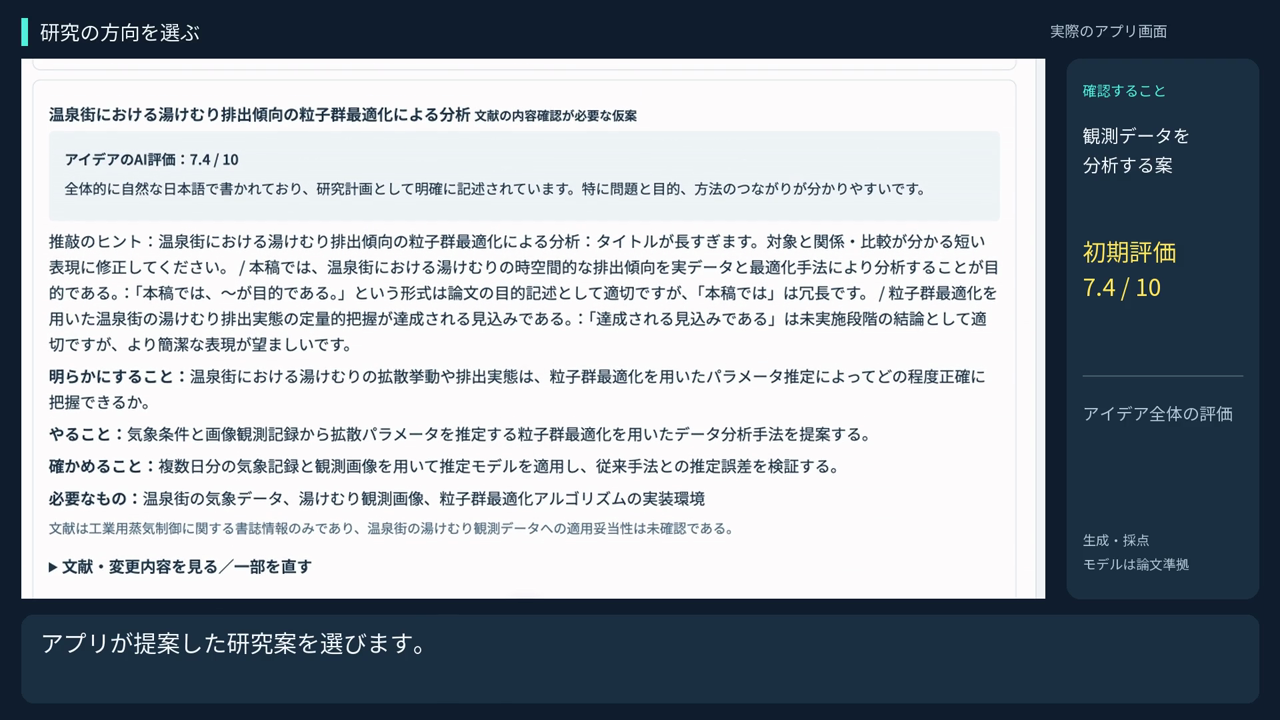
\includegraphics[width=\paperwidth,height=\paperheight]{assets/buildabstract-demo-poster.png}};
 \node[rounded corners=2mm,fill=black,fill opacity=.78,text opacity=1,inner xsep=9mm,inner ysep=4mm]
  at (current page.center) {%
   {\color{white}\fontsize{15}{18}\selectfont\bfseries ▶ 1分デモを全画面で再生}};
 \node[fill=black,fill opacity=.70,text opacity=1,inner xsep=5mm,inner ysep=2.2mm]
  at ([yshift=7mm]current page.south) {{\color{white}\fontsize{8}{10}\selectfont Build Abstract：問いの入力から研究計画の生成・評価まで}};
\end{tikzpicture}
\end{frame}

\begin{frame}[t]
\head{英語論文は書けなくても、バイトも恋愛もしてWI26まで届きました}{04}{WI26の事例}
\pair{研究一色ではない日常}{
 \bigtext{普通の学生生活も忙しい}
 \bullets{
  \lineitem{三重総合高校出身}
  \lineitem{ドンキでアルバイト}
  \lineitem{シーシャバーでもアルバイト}
  \lineitem{彼女と別れたり、新しくできたり}
  \lineitem{英語論文は自力では読み書きできない}}
}{AIを研究工程に入れた結果}{
 \bigtext{WI26フルペーパー採択}
 \bullets{
  \lineitem{テーマ設定はわりと順調}
  \lineitem{Codexへ指示して実装・実験}
  \lineitem{英語論文の読解と原稿作成はAI}
  \lineitem{教員・共著者が直接修正して完成}}
 \vspace{1.8mm}
 \begin{columns}[T,totalwidth=\linewidth]
  \begin{column}{.31\linewidth}
   \begingroup\setlength{\fboxsep}{.5mm}\setlength{\fboxrule}{.35pt}%
   \fbox{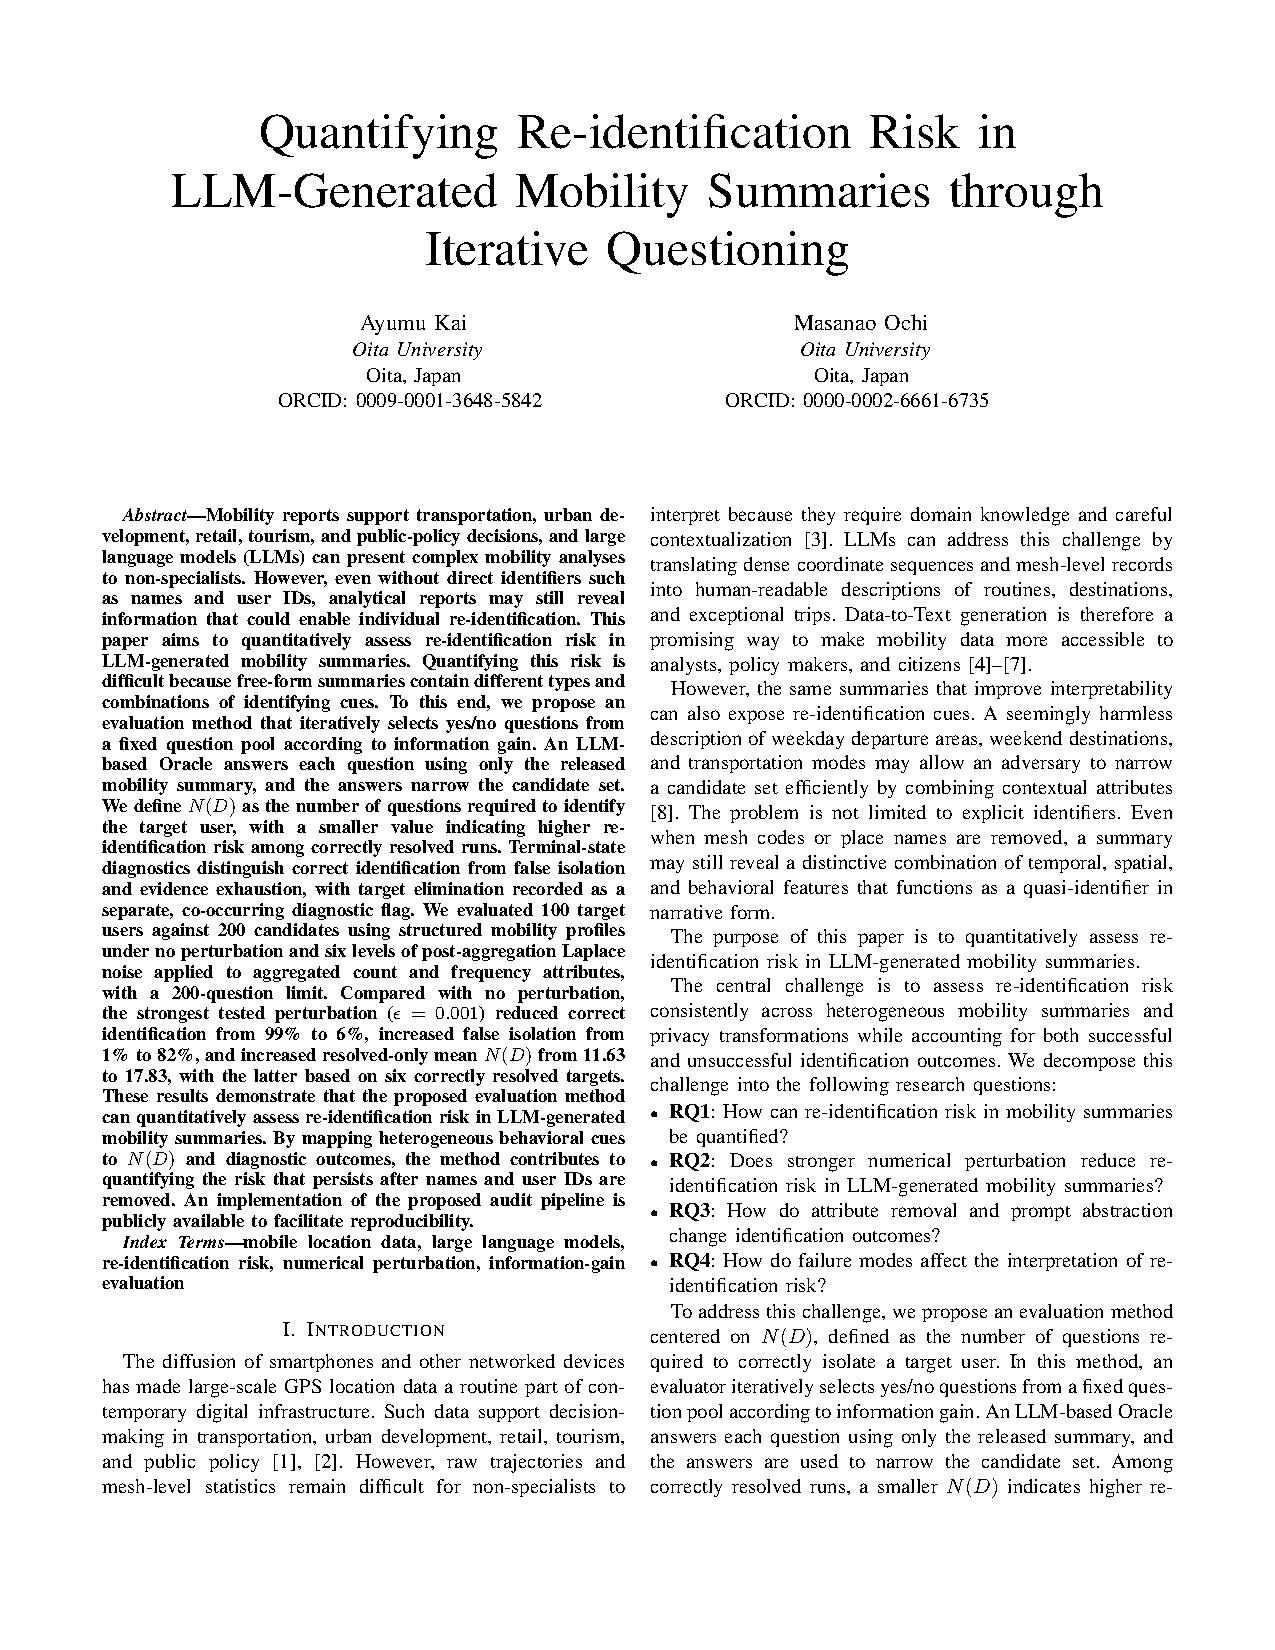
\includegraphics[page=1,width=\dimexpr\linewidth-1.7mm\relax]{assets/wi26-paper.pdf}}\endgroup
  \end{column}
  \begin{column}{.65\linewidth}
   {\color{Past}\fontsize{8.2}{10}\selectfont\bfseries Highly Novel Contribution\par}
   \vspace{1mm}
   {\fontsize{8}{10.5}\selectfont
    ``a fundamentally new approach''\par
    \vspace{1mm}
    ``a significant conceptual advance''\par}
   \vspace{1.5mm}
   \smalltext{逐次質問で再識別リスクを測る発想を、査読者が最も強く評価。}
  \end{column}
 \end{columns}
}
\bridge{研究だけに集中できる学生を待たず、普通の生活の中で研究を完成できる工程にする。}
\end{frame}

\begin{frame}[t]
\head{LLMの移動要約を、Akinator式の質問で再識別できるか測りました}{04}{WI26論文の中身}
\pair{提案アルゴリズム：$N(D)$}{
 \bigtext{少ない質問ほど危ない}
 \bullets{
  \lineitem{位置履歴を構造化し、LLMで文章要約}
  \lineitem{候補者200人と質問プールを用意}
  \lineitem{情報利得が最大の質問を選ぶ}
  \lineitem{LLM Oracleが要約だけを見て回答}
  \lineitem{正しく1人に絞るまでの質問数が$N(D)$}}
 \visual{wi26-algorithm.png}{18mm}{WI26論文の提案手法}
 \smalltext{A. Kai and M. Ochi, WI26, Fig.~1}
}{数値摂動で再識別を抑える}{
 \bigtext{正しく特定：99人 → 6人}
 \bullets{
  \lineitem{対象100人、候補200人、最大200質問}
  \lineitem{未加工では99人を正しく特定}
  \lineitem{$\epsilon=0.001$では正解6人、誤分離82人}
  \lineitem{成功例の平均$N(D)$：11.63 → 17.83}
  \lineitem{強い摂動ほど全体の特定成功率は低下}}
 \visual{wi26-results.png}{24mm}{数値摂動と再識別結果}
 \smalltext{Fig.~2。17.83は正しく特定できた6人のみの平均。}
}
\end{frame}

\begin{frame}[t]
\head{AIで英語を書いても、査読者が評価したのは新規性と評価設計でした}{04}{査読コメント}
\pair{実際に褒められたところ}{
 {\color{Past}\fontsize{10.5}{13}\selectfont\bfseries Highly Novel Contribution\par}
 \smalltext{``a fundamentally new approach'' --- sequential questioningで自由記述の再識別リスクを測る点を、significant conceptual advanceと評価。}
 \vspace{2.5mm}
 {\color{Past}\fontsize{10.5}{13}\selectfont\bfseries Rigorous Technical Framework\par}
 \smalltext{``mathematically sound'' --- 候補選択、情報利得、終了条件が明確。$N(D)$と失敗診断を分けた点をparticularly thoughtfulと評価。}
 \vspace{2.5mm}
 {\color{Past}\fontsize{10.5}{13}\selectfont\bfseries Comprehensive Experimental Design\par}
 \smalltext{複数のプライバシー保護条件を、同じ監査手順で系統的に比較した点を評価。}
}{何が新規性になったか}{
 \bigtext{結果より「測り方」}
 \bullets{
  \lineitem{固有表現検出や静的な匿名性指標から離れた}
  \lineitem{攻撃者が質問を重ねる過程をモデル化した}
  \lineitem{成功時だけ$N(D)$を定義し、失敗を別に記録}
  \lineitem{誤分離、真の候補除外、情報枯渇を区別}
  \lineitem{数値摂動、属性除去、要約抽象度を比較}
  \lineitem{AIが書いた英語でも、評価対象は研究設計}}
}
\bridge{英語を作る工程はAIで短縮できる。それでも、新しい問いと検証可能な評価設計がなければ査読は通らない。}
\end{frame}

\begin{frame}[t]
\head{成果物と実行環境を共有すると、本人が消えても引き継げます}{04}{GitHubと共有サーバ}
\pair{平時から同じ場所で作業}{
 \bigtext{引き継げる状態を常設する}
 \bullets{
  \lineitem{サーバ上の共有作業ディレクトリを必須にする}
  \lineitem{LaTeX、PDF、コード、データ、ログを同居させる}
  \lineitem{節目ごとにGitHubへcommit・push}
  \lineitem{ブランチと履歴に変更過程を残す}
  \lineitem{別の人が同じ環境から再開できる}}
 \vspace{2mm}
 {\color{Past}\fontsize{10.5}{13}\selectfont\bfseries 締切日に本人が消えたら\par}
 \bullets{
  \lineitem{大知がサーバへログイン}
  \lineitem{Git履歴、コード、結果をCodexで調査}
  \lineitem{実験を続け、論文を直し、そのまま投稿}}
}{実際の作業画面}{
 \bigtext{全部が一画面に見える}
 \visual{shared-research-workspace.png}{43mm}{VS Code上の共有研究環境}
 \smalltext{左：リポジトリ／中央：論文PDF／右：AgentとGitHub同期／下：サーバ上のターミナル}
}
\bridge{GitHubとサーバに残すのは成果物と実行環境。締切日の引き継ぎ資料にもなる。}
\end{frame}

\begin{frame}[t]
\head{次はAgentへの指示まで共有し、学生・大知・AIを同じ場に置く}{05}{Buzz：指示履歴の共有}
\pair{会話も研究記録にする}{
 \bigtext{委任の過程を残す}
 \bullets{
  \lineitem{研究テーマごとに共有チャンネルを作る}
  \lineitem{学生が@Agentで作業を指示}
  \lineitem{Agentが実装内容と変更理由を返信}
  \lineitem{テスト、GitHub反映、公開まで報告する}
  \lineitem{大知が判断と結果をリアルタイムで見る}
  \lineitem{必要な箇所だけ介入して追加指示を出す}}
 \vspace{2mm}
 \smalltext{個人とAgentの会話を、研究室から見える作業ログへ変える。}
}{指示そのものが見える}{
 \bigtext{作業の実況を共有する}
 \visual{buzz-shared-agent.png}{43mm}{Buzz上の学生・大知・AI Agentの共同作業}
 \smalltext{学生の指示 → Agentの実装報告 → テスト → GitHub・公開環境への反映まで同じスレッド。}
}
\bridge{GitHubとサーバは成果物を残す。Buzzは、誰が何を頼み、何を確認したかを残す。}
\end{frame}

\begin{frame}[plain]
\begin{tikzpicture}[remember picture,overlay]
 \node[inner sep=0] at (current page.center) {%
  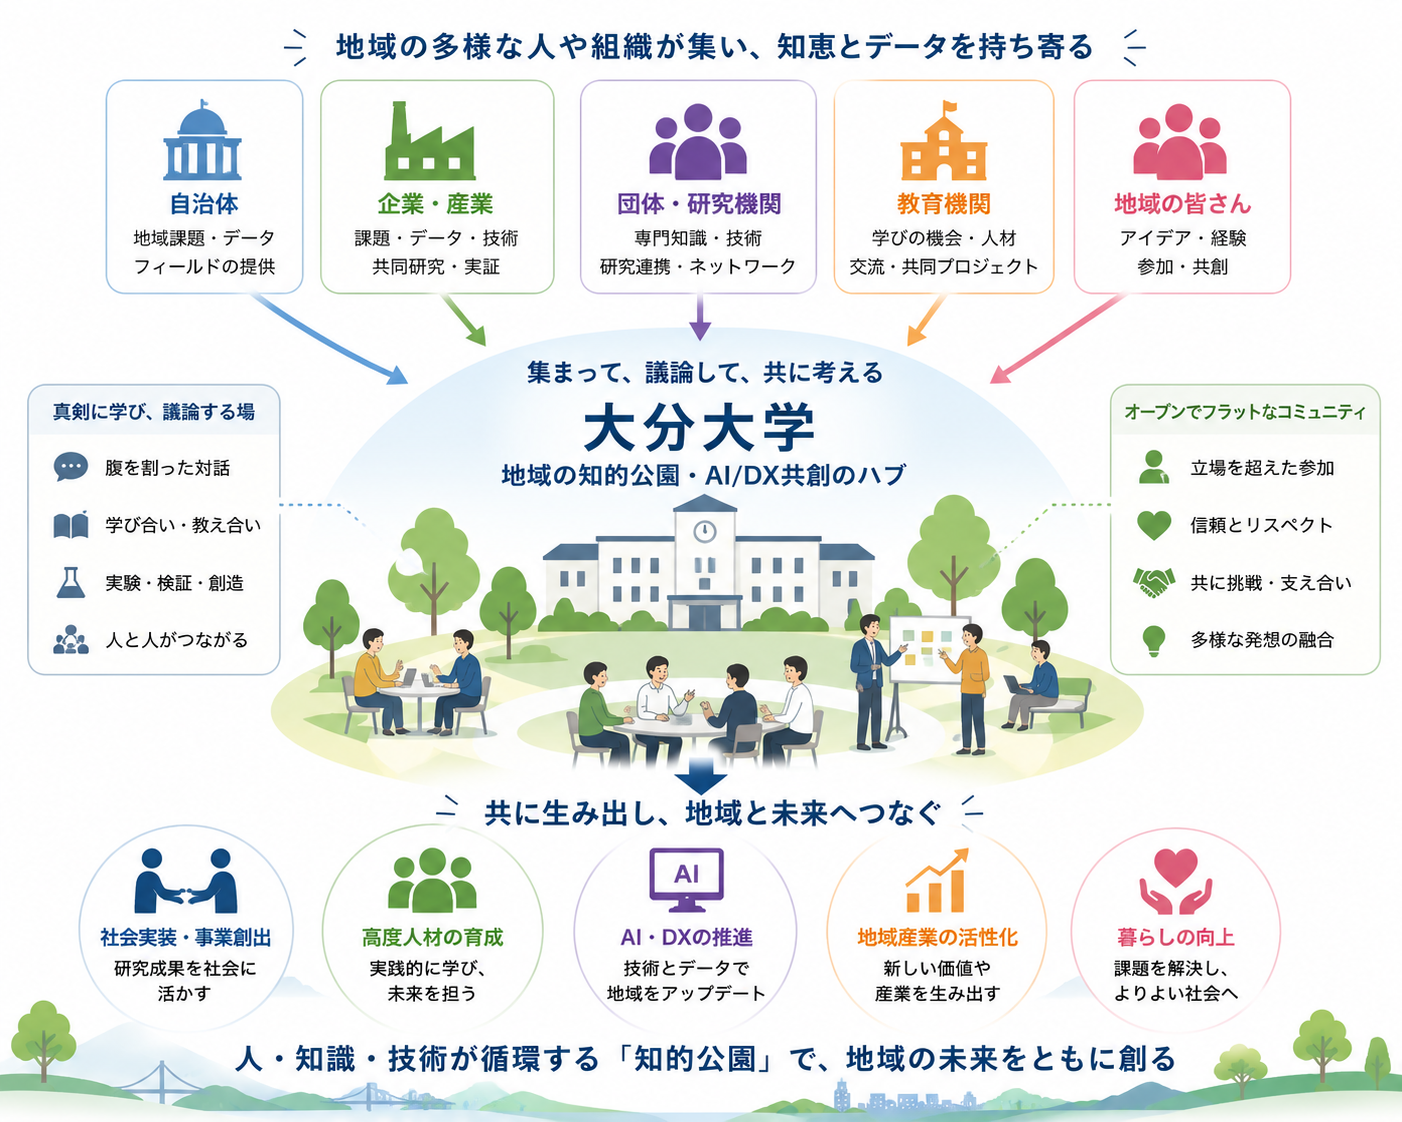
\includegraphics[height=\paperheight]{assets/poster-oita-hub.png}};
\end{tikzpicture}
\end{frame}

\end{document}
